\Section{Доменная система имён}{Лекции 5-6}{Игорь Смирнов}

У систем именования ресурсов есть несколько функций.

Основные:
\begin{itemize}
    \item Преобразование символических имен (какой-то удобной мнемоники для человека) в адреса
    \item Преобразование адресов в символические имена
\end{itemize}

Дополнительные:
\begin{itemize}
    \item Маршрутизация почты
    \item Хранение дополнительной информации об узлах
\end{itemize}

Когда интернет только появился, для именования узлов использовали таблицы соответствий.

Это был файл {\tt hosts}, в котором было соответствие имён и адресов. Первые сети так и работали.

Но такая схема долго прожить не смогла. Как только появлялся новый узел, он регистрировался и новый файл hosts рассылался всем. Это неудобно. И информация постоянно меняется.

Предложили выход~--- распределённую базу данных соответствий.

Таким образом была разработана система DNS.

Основные особенности:
\begin{itemize}
    \item Распределённая по Internet база данных имён
    \item Иерархическое именование ресурсов
    \item Распределенные по сети серверы DNS, осуществляющие запросы к распределенной базе данных DNS
\end{itemize}

Система DNS~--- это дерево. У него есть корень, который называется <<.>>. Внутрь домена верхнего уровня могут вкладываться домены следующего уровня. Количество уровней иерархии~--- неограниченно. Полное имя узла получается восстановлением по дереву снизу вверх цепочки имен доменов, разделенных точками.

Любое правильное имя в сети Internet должно заканчиваться на точку. Но почти всегда можно точку не писать.

\Subsection{Доменные имена}

Иерархия имён в DNS:

\begin{figure}[H]
  \centering
  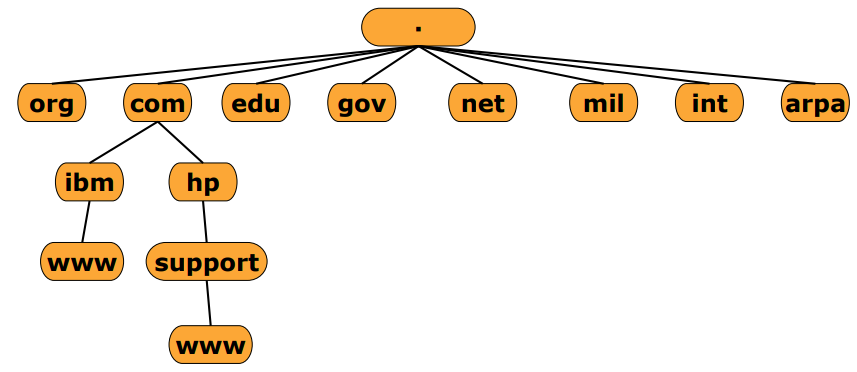
\includegraphics[width=15cm]{images/05/01}
\end{figure}

arpa~--- устаревший домен, используется для управления в Internet.

После того как интернет перестал быть американским, были добавлены национальные домены первого уровня (двухбуквенные country-коды). Например, {\tt fr, de, ca, ru, uk, ua, su (Soviet Union!)}.

{\bf Кулыстори.} Есть домен {\tt tv} и он принадлежит Тувалу. Основной доход Тувалу~--- сдача домена tv под использование телевизионным компаниям.

Изначально us и su были географическими доменами. Идея была такая: в других доменах можно заводить поддомены как хотите, а в этих только с географическим принципом. Например, в us поддомены~--- названия штатов, а у них поддомены~--- названия городов. То есть если хотите обратиться в мэрию Нью-Йорка, думать не надо, просто вбиваете {\tt gov.ny.us}.

Но теперь в домене su можно регистрировать что угодно.

А ещё появились дополнительные домены первого уровня (asia, aero, biz, cat (нет, не для котеек, а для каталанского языкового и культурного сообщества), eco, info, museum, name, travel ...)

Несколько лет назад было принято решение снять ограничения с регистрации доменов первого уровня.

В том числе, это ограничение сняли из-за того, что слишком много всего было на домене {\tt com}.

Но некоторые имена всё-таки нельзя использовать в качестве доменов:
\begin{itemize}
    \item example~--- зарезервировано для примеров (например, на лекциях) 
    \item invalid~--- зарезервировано для использования в очевидно неверных именах доменов 
    \item localhost~--- зарезервировано для того чтобы избежать конфликтов с традиционным использованием localhost
    \item test — зарезервировано для использования в тестах
    \item * local, * localdomain для адресов, применяемых в пределах одной машины или локальной компьютерной сети
\end{itemize}

\Subsubsection{Правила построения доменных имён}

Используемые символы:
\begin{itemize}
    \item Строчные латинские символы
    \item Цифры
    \item Знак <<->>
\end{itemize}

Все остальные символы запрещены. Заглавные латинские символы интерпретируются как строчные.

Но национальные алфавиты использовать можно (стопкоронавирус.рф). Это делается с помощью системы IDN. На самом деле это просто синтаксический сахар. Просто перекодировка Unicode в DNS (ACE-кодировка).

\Subsection{Устройство DNS}

Компоненты DNS:
\begin{itemize}
    \item DNS-серверы~--- специальное программное обеспечение, которое обеспечивает трансляцию из имён в адреса и наоборот
    \item Клиентские программы~--- программы, которые используют имена, а не адреса. Браузер, почта
    \item Resolvers~--- обеспечивают клиентским программам сервис для использования DNS
\end{itemize}

\begin{figure}[H]
  \centering
  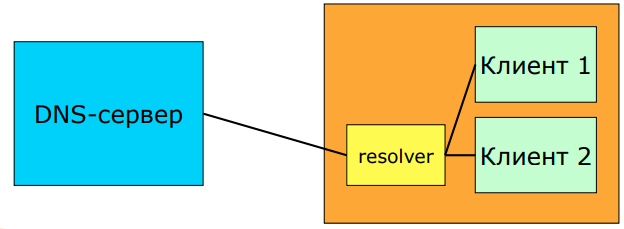
\includegraphics[width=15cm]{images/05/02}
\end{figure}

\Subsubsection{Организация DNS и прямой поиск}

Всё дерево имен поделено на участки ответственности~--- зоны.

Для каждой зоны существует свой сервер DNS, отвечающий за зону. Сервер, отвечающий за зону~--- авторитетный сервер.

Для каждой зоны должно быть несколько авторитетных серверов: один~--- первичный (содержит исходную информацию о зоне), несколько вторичных (содержат копию информации о зоне и периодически обновляют информацию).

Все сервера хранят информацию о зоне, обслуживают запросы об этой зоне, перенаправляют запросы о других зонах вышестоящим или подчиненным серверам. Существенная часть серверов (но не все!) занимается кэшированием информации о других зонах.

Первичные серверы копирую зонную информацию вторичным и модифицируют первичную информацию.

Вторичные серверы периодически опрашивают первичных.

Типы DNS серверов по способу ответа на запрос:
\begin{itemize}
    \item Рекурсивные серверы
    \begin{itemize}
        \item Самостоятельно выполняют весь поиск (если они не ответственны за эту зону)
        \item Кэшируют полученную информацию
    \end{itemize}
    \item Нерекурсивные серверы
    \begin{itemize}
        \item Указывают, где есть необходимая информация
        \item Не кэшируют информацию
    \end{itemize}
\end{itemize}

Чем ближе сервер к клиенту, тем больше вероятность, что он рекурсивный.

Все серверы первого уровня~--- нерекурсивные.

У каждого компьютера сконфигурирован DNS-сервер по умолчанию.

Пусть мы хотим обратиться к сайту spb.hse.ru.

Ресолвер смотрит, нет ли у него информации. Если нет~--- обращается к DNS-серверу по умолчанию. Тот смотрит, нет ли у него информации. Если нет, то обращается к одному из корневых серверов (их всего 13 штук и о них позже). Он нерекурсивный, поэтому возвращает нам адрес того, где нужно искать и мы сами обращаемся по тому адресу. Ну и так далее, пока не найдётся нужное имя.

Это называется процедурой прямого поиска.

{\bf Корневые серверы.}

Их 13 штук. На территории России и Африки нет ни одного.

К корневому серверу очень большой трафик.

Например, в Москве сделали зеркало корневого сервера. Провайдеры перехватывают запросы к корневым серверам и перепосылают его на зеркало, экономя трафик.

Кстати, в корпоративной сети РЖД несколько миллионов компьютеров, они подняли свой DNS со своим корневым доменом.

Вся база данных DNS состоит из ресурсных записей (RR).

Дальнейший рассказ будет использовать терминологию системы bind (Berkeley Internet Name Domain)~--- это ведущий name-сервер в мире и его терминология используется повсеместно.

Каждая запись хранит определённый тип информации и содержит следующие поля:
\begin{itemize}
    \item Имя (необязательное). В случае отсутствия используется предыдущее
    \item Класс записи (для Интернета - IN)
    \item Тип записи
    \item Время актуальности (необязательное). В случае отсутствия используется значение по умолчанию. Сколько данную запись можно держать в кэше
    \item Параметры записи (зависят от типа)
\end{itemize}

Существует несколько типов записей.

{\bf Адресная запись.}

Подавляющее число записей имеют этот тип.

Обозначается <<A>>

Параметры:
\begin{itemize}
    \item Доменное имя узла
    \item Соответствующий адрес
\end{itemize}
Формат bind:
\begin{itemize}
    \item name IN A address
\end{itemize}
Пример: {\tt school IN A 195.19.212.16}

Обратим внимание, что здесь нет точки. Это относительный адрес. Это означает, что подразумевается домен по умолчанию для этого DNS-сервера

{\bf Запись о сервере имён.}

Обозначается <<NS>>

Позволяет задать вторичный сервер имён

Параметры:
\begin{itemize}
    \item Имя домена
    \item Адрес сервера имён
\end{itemize}
Формат bind:
\begin{itemize}
    \item domain IN NS address
\end{itemize}
Пример: {\tt school.server.ru. IN NS 195.19.212.13}

Для домена {\tt school.server.ru.} указали, что у него есть вторичный DNS-сервер по такому-то адресу.

Как минимум одна такая запись должна быть в домене.

 {\bf Главная ресурсная запись.}

 Обозначается <<SOA>> (start of authority)

 Описывает основные параметры зоны.

 Параметры:
 \begin{itemize}
    \item Имя домена
    \item Имя первичного DNS-сервера (вторичный задаётся через запись NS)
    \item Почтовый адрес администратора
    \item Серийный номер зоны (Serial)~--- уникальный идентификатор, который увеличивается по мере изменения зоны. Является ключом для вторичного сервера. Если вторичный сервер видит, что идентификатор изменился, то он понимает, что зона изменилась и зону нужно скопировать 
    \item Период обновления (Refresh)~--- как часто вторичный сервер должен обращаться за изменением информации
    \item Время валидности данных зоны (Expire)~--- как долго вторичный сервер будет отвечать на доменные запросы, если первичный не отвечает
    \item Период повторных попыток (Retry)~--- период повторных попыток вторичного обратиться к первичному, если первичный не ответил.
    \item Значение по умолчанию (DefaultTTL)~--- дефолтное время кэширования для всех записей в зоне
\end{itemize}

Должна быть одна на зону.

Формат bind: {\tt domain IN SOA ns e-mail (Serial Refresh Retry Expire DefaultTTL)}

Пример: {\tt school.server.ru. IN SOA ns.school.server.ru. admin.school.server.ru. (2008121801 3600 900 2592000 900)}

Домен {\tt school.server.ru.}. У него есть первичный сервер. Адрес почты администратора~--- {\tt admin@school.rerver.ru} (собака зарезервирована).

Запись скорее всего от 18 декабря 2008 года, номер изменения 01. Так администраторы часто ведут зону.

Refresh~--- раз в час. Retry~--- 15 минут. Expire~--- месяц. DefaultTTL~--- 15 минут.

При запросе копии зоны вторичным сервером используется тип передачи AXFR (о том, что это такое~--- позже).

Этих трёх записей достаточно для функционирования DNS. Но у DNS есть и дополнительные функции.

{\bf Запись о сервере электронной почты}

Обозначается <<MX>>

Параметры:
 \begin{itemize}
    \item Имя почтового домена
    \item Имя почтового сервера
    \item Приоритет
\end{itemize}

Формат bind: {\tt Mail-domain IN MX priority address}

Пример: \\
{\tt office IN MX 10 mail.school.server.ru.}\\
{\tt office IN MX 20 mail.yandex.ru.}

Если кто-то послал почту по адресу {\tt xxx@office.ИМЯНАШЕГОДОМЕНА}. Посылаем сначала на первый, а если он вдруг не отвечает, то на второй.

{\bf Запись о псевдониме.}

Обозначается <<CNAME>>

Параметры:
\begin{itemize}
    \item Доменное имя узла (псевдоним)
    \item Реальное (каноническое имя)
\end{itemize}

Формат bind: {\tt сname IN CNAME name}

Пример: {\tt www IN CNAME node.school.server.ru.}

Если кто-то обратится по адресу {\tt www.ИМЯНАШЕГОДОМЕНА}, на самом деле это превратится в адрес {\tt node.sschool.server.ru.}

Псевдонимы запрещены при маршрутизации почты.

{\bf Запись о сервисе.}

Обозначается <<SRV>>.

Формат bind: {\tt \_Service.\_Proto.Name IN SRV Priority Weight Port Target}

Параметры:
\begin{itemize}
    \item Service~--- имя сервиса
    \item Proto~--- имя протокола
    \item Priority~--- приоритет
    \item Weight~--- вес (для балансировки нагрузки). Доля запросов, которые пойдут на этот сервис
    \item Target~--- имя узла, на котором находится сервис
\end{itemize}

Пример:\\
{\tt \_xmpp-server.\_tcp.example.ru. 3600 IN SRV 20 0 5269 jabber1.ru.}\\
{\tt \_xmpp-client.\_tcp.example.ru. 3600 IN SRV 20 90 5222 jabber1.ru.}\\
{\tt \_xmpp-client.\_tcp.example.ru. 3600 IN SRV 20 10 5222 jabber2.ru.}

Здесь показан способ балансировки нагрузки нагрузки. 90\% запросов будут идти к первому клиенту, а 10\% ко второму.

Через запись SRV можно полностью повторить запись MX.

{\bf Другие ресурсные записи}
\begin{itemize}
    \item WKS~--- анонсирование сервисов~--- сообщает, какие сервисы запущены на данном узле. Не используется, так как использовалась хакерами
    \item HINFO~--- информация об узле. Опять мечта для хакера.
    \item RP~--- Responsable Person~--- почтовый адрес ответственного за узел, но эту запись никто не заполнял и она не используется.
    \item TXT~--- текстовая запись. Раньше: <<Любая дополнительная текстовая информация, которую вы хотите сообщит миру о своём узле>>. Сейчас: <<Запись, куда можно поместить любую информацию об узле. В том числе, автоматически обрабатываемую.>>. Используется. Могут размешаться, например, открытые ключи.
    \item ...
\end{itemize}

\Subsubsection{Обратный поиск}

Хотим по IP-адресу узнать доменное имя. 

Цель следующая: убедиться, что адрес валидный и на него зарегистрировано доменное имя. Используется в целях безопасности.

Используются механизмы прямого поиска. Для этого введён специальный домен: {\tt in-addr.arpa.}. Имена состоят из октетов IP-адресов.

При запросу имени для адреса X.Y.Z.T строится запрос для
имени: {\tt T.Z.Y.X.in-addr.arpa} и такой запрос обслуживается как прямой.

Пример:\\
Адрес {\tt 195.19.212.97}\\
Доменное имя: {\tt 97.212.19.195.in-addr.arpa.}

Введена ресурсная запись PTR

Используется для преобразования имён из домена in-addr.arpa. в доменное имя.

Параметры:
\begin{itemize}
    \item Имя узла в домене in-addr.arpa.
    \item Доменное имя узла
\end{itemize}

Формат bind: {\tt in-addr-name IN PTR name}

Примеры:\\
{\tt 11.12.19.195.in-addr.arpa. IN PTR ya.ru}\\
{\tt 16 IN PTR office.school.server.ru}

\Subsection{Система bind}

Организация базы данных DNS.
\begin{itemize}
    \item Главный файл конфигурации {\tt /etc/named.conf}
    \item Файл прямого преобразования {\tt /var/named/ftk.hosts}
    \item Файл обратного преобразования {\tt /var/named/ftk.rev}
    \item Файл кэша корневых серверов {\tt /var/named/named.ca}
    \item Файл обратного преобразования локальной зоны {\tt /var/named/local.rev}~--- чтобы {\tt 127.0.0.1} преобразовывалось в {\tt localhost}
\end{itemize}

\Subsection{Расширения DNS}

\Subsubsection{Динамические обновления}

Существуют динамические системы управления адресами (DHCP) (динамическая смена IP-шника). И те, кто ими пользуются, при получении нового IP, хотят иметь старое доменное имя.

Идея: авторизованный клиент (например, DHCP сервер) посылает серверу DNS запрос на изменение ресурсной записи. Если сервер не первичный, запрос пересылается наверх, пока запрос не дойдёт до первичного. Когда запрос дошёл до первичного сервера, тот заносит информацию в свою БД, инкрементирует номер зоны, а вторичные серверы потом это подхватят.

\Subsubsection{Нотификация}

Асинхронное информирование об изменении информации~--- технология DNS NOTIFY.

Первичный сервер посылает сообщение <<У меня есть обновление!>> всем известным ему вторичным, вторичные посылают всем другим вторичным (редко бывает, что первичный не знает обо всех вторичных, но такое встречается). Каждое сообщение от первичного подтверждается. Вторичные осуществляют запрос зоны как при периодическом обновлении.

\Subsubsection{Инкрементальная передача зон}

При частом обновлении информации слишком много трансферов зон. Поэтому придумали пересылать не всю зону, а только то, что изменилось.

Вторичный посылает свой серийный номер зоны, первичный считает дельту и отправляет её.

Тип запроса~--- IXFR.

\Subsection{Ещё пару слов о DNS}

\Subsubsection{Серверы-ретрансляторы}

Их используют для сокращения внешнего трафика.

Пусть у нас много трафика. Выделим сервер-ретранслятор. Он не будет обслуживать никакую зону, а только обслуживает запросы наших серверов (принимает запросы от них и отсылает в интернет). И его кэш разделяется нашими серверами. Здорово экономит трафик.

Они кэшируют информацию всех запросов.

Должны конфигурироваться как ретрансляторы.

\Subsubsection{Утилиты конфигурирования}

\begin{itemize}
    \item nslookup
    \item dig
    \item host
\end{itemize}

\Subsubsection{Реализация DNS}

Для клиентских запросов и ответов используется UDP

Для зонных пересылок и клиентских запросов большого размера~--- TCP

И в UDP и в TCP порт 53

В настоящее время часто используется DNS с шифрованием.

\Subsubsection{Сосуществование различных систем именования}

В Windows сначала смотрим в Hosts, а уже потом в DNS (хакеры использовали это, подменяя Hosts).

В Unix приоритизация указывается в {\tt /etc/host.conf}

\Subsubsection{Регистрация доменных имён}

Есть море разных организаций. Например, в США это InterNIC, а в России RIPN

В домене ru управлением и поддержкой занимается RocНИИРОС (\url{ripn.net})

Они же поддерживают сервер whois~--- он позволяет сказать, на кого зарегистрирован домен.

Кроме того, есть координационный центр для доменов ru и рф (\url{cctld.ru}).

{\bf Кулстори.} Сама регистрация доменов изначально велась РосНИИРОС-ом, но 21 год назад ситуация изменилась. Раньше цена домена в домене ru была заоблачной. Это стоило 100\$ в год и 100\$ за ведение. Но Путин стал премьером, провёл совещание, на котором Артемий Лебедев прочитал огромный доклад, где заклеймил позором РосНИИРОС, мол во всех странах это стоит гораздо дешевле (ну стоит и стоит). Проблема практически сразу была решена и RIPN перестал быть регистратором доменов и стал делегировать свою функцию. Сейчас регистраторов 50 (\url{ccltd.ru/domain/reg/}).

{\bf Кулстори.} Сначала появились доменные адреса, а уже потом правительства стали думать о том, как вообще эти имена нужно регистрировать. И пока закона не было, появились киберсквотеры. Они скупали звучные доменные имена задёшево, а потом за большие деньги продавали их. Самый известный случай~--- с Microsoft. У них была Windows NT. Была Windows NT 3.5, Windows NT 4.0. А Windows NT 5.0 не было. Она стала Windows 2000. Билл Гейтс объявил это, а в течение часа умный молодой человек зарегистрировал на себя \url{windows2000.com} и перепродал Microsoft-у за 5 миллионов долларов.

{\bf Кулстори.} До гугла была поисковая система Altavista. И у неё был адрес \url{altavista.digital.com}. А адрес \url{altavista.com} прикарманила себе какая-то компания со своим простеньким поисковым движком. И они продали это имя Альтависте за большие деньги. 

Теперь есть законодательство, позволяющее обладателю товарного знака забирать такие имена.

{\bf Кулстори.} Когда в 2000-х годах мобильная связь только открывалась в России, МТС решила прийти в СПб. Для этого они решили выйти к нам под брендом <<Телеком 21>>. Киберсквотеры услышали это и в первый же день выкупили всё благозвучное с похожими именами и ждали предложений от МТС. А МТС зарегистрировались как \url{spb.mts.ru}.

\begin{figure}[h]
  \centering
  
\includegraphics[width=10cm]{images/05/03}
\end{figure}

